% Options for packages loaded elsewhere
\PassOptionsToPackage{unicode}{hyperref}
\PassOptionsToPackage{hyphens}{url}
\PassOptionsToPackage{dvipsnames,svgnames,x11names}{xcolor}
%
\documentclass[
  letterpaper,
  DIV=11,
  numbers=noendperiod]{scrartcl}

\usepackage{amsmath,amssymb}
\usepackage{lmodern}
\usepackage{iftex}
\ifPDFTeX
  \usepackage[T1]{fontenc}
  \usepackage[utf8]{inputenc}
  \usepackage{textcomp} % provide euro and other symbols
\else % if luatex or xetex
  \usepackage{unicode-math}
  \defaultfontfeatures{Scale=MatchLowercase}
  \defaultfontfeatures[\rmfamily]{Ligatures=TeX,Scale=1}
\fi
% Use upquote if available, for straight quotes in verbatim environments
\IfFileExists{upquote.sty}{\usepackage{upquote}}{}
\IfFileExists{microtype.sty}{% use microtype if available
  \usepackage[]{microtype}
  \UseMicrotypeSet[protrusion]{basicmath} % disable protrusion for tt fonts
}{}
\makeatletter
\@ifundefined{KOMAClassName}{% if non-KOMA class
  \IfFileExists{parskip.sty}{%
    \usepackage{parskip}
  }{% else
    \setlength{\parindent}{0pt}
    \setlength{\parskip}{6pt plus 2pt minus 1pt}}
}{% if KOMA class
  \KOMAoptions{parskip=half}}
\makeatother
\usepackage{xcolor}
\setlength{\emergencystretch}{3em} % prevent overfull lines
\setcounter{secnumdepth}{-\maxdimen} % remove section numbering
% Make \paragraph and \subparagraph free-standing
\ifx\paragraph\undefined\else
  \let\oldparagraph\paragraph
  \renewcommand{\paragraph}[1]{\oldparagraph{#1}\mbox{}}
\fi
\ifx\subparagraph\undefined\else
  \let\oldsubparagraph\subparagraph
  \renewcommand{\subparagraph}[1]{\oldsubparagraph{#1}\mbox{}}
\fi

\usepackage{color}
\usepackage{fancyvrb}
\newcommand{\VerbBar}{|}
\newcommand{\VERB}{\Verb[commandchars=\\\{\}]}
\DefineVerbatimEnvironment{Highlighting}{Verbatim}{commandchars=\\\{\}}
% Add ',fontsize=\small' for more characters per line
\usepackage{framed}
\definecolor{shadecolor}{RGB}{241,243,245}
\newenvironment{Shaded}{\begin{snugshade}}{\end{snugshade}}
\newcommand{\AlertTok}[1]{\textcolor[rgb]{0.68,0.00,0.00}{#1}}
\newcommand{\AnnotationTok}[1]{\textcolor[rgb]{0.37,0.37,0.37}{#1}}
\newcommand{\AttributeTok}[1]{\textcolor[rgb]{0.40,0.45,0.13}{#1}}
\newcommand{\BaseNTok}[1]{\textcolor[rgb]{0.68,0.00,0.00}{#1}}
\newcommand{\BuiltInTok}[1]{\textcolor[rgb]{0.00,0.23,0.31}{#1}}
\newcommand{\CharTok}[1]{\textcolor[rgb]{0.13,0.47,0.30}{#1}}
\newcommand{\CommentTok}[1]{\textcolor[rgb]{0.37,0.37,0.37}{#1}}
\newcommand{\CommentVarTok}[1]{\textcolor[rgb]{0.37,0.37,0.37}{\textit{#1}}}
\newcommand{\ConstantTok}[1]{\textcolor[rgb]{0.56,0.35,0.01}{#1}}
\newcommand{\ControlFlowTok}[1]{\textcolor[rgb]{0.00,0.23,0.31}{#1}}
\newcommand{\DataTypeTok}[1]{\textcolor[rgb]{0.68,0.00,0.00}{#1}}
\newcommand{\DecValTok}[1]{\textcolor[rgb]{0.68,0.00,0.00}{#1}}
\newcommand{\DocumentationTok}[1]{\textcolor[rgb]{0.37,0.37,0.37}{\textit{#1}}}
\newcommand{\ErrorTok}[1]{\textcolor[rgb]{0.68,0.00,0.00}{#1}}
\newcommand{\ExtensionTok}[1]{\textcolor[rgb]{0.00,0.23,0.31}{#1}}
\newcommand{\FloatTok}[1]{\textcolor[rgb]{0.68,0.00,0.00}{#1}}
\newcommand{\FunctionTok}[1]{\textcolor[rgb]{0.28,0.35,0.67}{#1}}
\newcommand{\ImportTok}[1]{\textcolor[rgb]{0.00,0.46,0.62}{#1}}
\newcommand{\InformationTok}[1]{\textcolor[rgb]{0.37,0.37,0.37}{#1}}
\newcommand{\KeywordTok}[1]{\textcolor[rgb]{0.00,0.23,0.31}{#1}}
\newcommand{\NormalTok}[1]{\textcolor[rgb]{0.00,0.23,0.31}{#1}}
\newcommand{\OperatorTok}[1]{\textcolor[rgb]{0.37,0.37,0.37}{#1}}
\newcommand{\OtherTok}[1]{\textcolor[rgb]{0.00,0.23,0.31}{#1}}
\newcommand{\PreprocessorTok}[1]{\textcolor[rgb]{0.68,0.00,0.00}{#1}}
\newcommand{\RegionMarkerTok}[1]{\textcolor[rgb]{0.00,0.23,0.31}{#1}}
\newcommand{\SpecialCharTok}[1]{\textcolor[rgb]{0.37,0.37,0.37}{#1}}
\newcommand{\SpecialStringTok}[1]{\textcolor[rgb]{0.13,0.47,0.30}{#1}}
\newcommand{\StringTok}[1]{\textcolor[rgb]{0.13,0.47,0.30}{#1}}
\newcommand{\VariableTok}[1]{\textcolor[rgb]{0.07,0.07,0.07}{#1}}
\newcommand{\VerbatimStringTok}[1]{\textcolor[rgb]{0.13,0.47,0.30}{#1}}
\newcommand{\WarningTok}[1]{\textcolor[rgb]{0.37,0.37,0.37}{\textit{#1}}}

\providecommand{\tightlist}{%
  \setlength{\itemsep}{0pt}\setlength{\parskip}{0pt}}\usepackage{longtable,booktabs,array}
\usepackage{calc} % for calculating minipage widths
% Correct order of tables after \paragraph or \subparagraph
\usepackage{etoolbox}
\makeatletter
\patchcmd\longtable{\par}{\if@noskipsec\mbox{}\fi\par}{}{}
\makeatother
% Allow footnotes in longtable head/foot
\IfFileExists{footnotehyper.sty}{\usepackage{footnotehyper}}{\usepackage{footnote}}
\makesavenoteenv{longtable}
\usepackage{graphicx}
\makeatletter
\def\maxwidth{\ifdim\Gin@nat@width>\linewidth\linewidth\else\Gin@nat@width\fi}
\def\maxheight{\ifdim\Gin@nat@height>\textheight\textheight\else\Gin@nat@height\fi}
\makeatother
% Scale images if necessary, so that they will not overflow the page
% margins by default, and it is still possible to overwrite the defaults
% using explicit options in \includegraphics[width, height, ...]{}
\setkeys{Gin}{width=\maxwidth,height=\maxheight,keepaspectratio}
% Set default figure placement to htbp
\makeatletter
\def\fps@figure{htbp}
\makeatother

\KOMAoption{captions}{tableheading}
\makeatletter
\makeatother
\makeatletter
\makeatother
\makeatletter
\@ifpackageloaded{caption}{}{\usepackage{caption}}
\AtBeginDocument{%
\ifdefined\contentsname
  \renewcommand*\contentsname{Table of contents}
\else
  \newcommand\contentsname{Table of contents}
\fi
\ifdefined\listfigurename
  \renewcommand*\listfigurename{List of Figures}
\else
  \newcommand\listfigurename{List of Figures}
\fi
\ifdefined\listtablename
  \renewcommand*\listtablename{List of Tables}
\else
  \newcommand\listtablename{List of Tables}
\fi
\ifdefined\figurename
  \renewcommand*\figurename{Figure}
\else
  \newcommand\figurename{Figure}
\fi
\ifdefined\tablename
  \renewcommand*\tablename{Table}
\else
  \newcommand\tablename{Table}
\fi
}
\@ifpackageloaded{float}{}{\usepackage{float}}
\floatstyle{ruled}
\@ifundefined{c@chapter}{\newfloat{codelisting}{h}{lop}}{\newfloat{codelisting}{h}{lop}[chapter]}
\floatname{codelisting}{Listing}
\newcommand*\listoflistings{\listof{codelisting}{List of Listings}}
\makeatother
\makeatletter
\@ifpackageloaded{caption}{}{\usepackage{caption}}
\@ifpackageloaded{subcaption}{}{\usepackage{subcaption}}
\makeatother
\makeatletter
\@ifpackageloaded{tcolorbox}{}{\usepackage[many]{tcolorbox}}
\makeatother
\makeatletter
\@ifundefined{shadecolor}{\definecolor{shadecolor}{rgb}{.97, .97, .97}}
\makeatother
\makeatletter
\makeatother
\ifLuaTeX
  \usepackage{selnolig}  % disable illegal ligatures
\fi
\IfFileExists{bookmark.sty}{\usepackage{bookmark}}{\usepackage{hyperref}}
\IfFileExists{xurl.sty}{\usepackage{xurl}}{} % add URL line breaks if available
\urlstyle{same} % disable monospaced font for URLs
\hypersetup{
  pdftitle={Quarto},
  pdfauthor={Le Nhat Tung},
  colorlinks=true,
  linkcolor={blue},
  filecolor={Maroon},
  citecolor={Blue},
  urlcolor={Blue},
  pdfcreator={LaTeX via pandoc}}

\title{Quarto}
\author{Le Nhat Tung}
\date{18/05/2023}

\begin{document}
\maketitle
\ifdefined\Shaded\renewenvironment{Shaded}{\begin{tcolorbox}[frame hidden, borderline west={3pt}{0pt}{shadecolor}, interior hidden, enhanced, breakable, boxrule=0pt, sharp corners]}{\end{tcolorbox}}\fi

\begin{center}\rule{0.5\linewidth}{0.5pt}\end{center}

\begin{Shaded}
\begin{Highlighting}[]
\InformationTok{\textasciigrave{}\textasciigrave{}\textasciigrave{}\{r\}}
\FunctionTok{setwd}\NormalTok{(}\StringTok{"C:/Users/Windows/RRcourse2023/Quarto\_Exercise\_2/"}\NormalTok{)}
\InformationTok{\textasciigrave{}\textasciigrave{}\textasciigrave{}}
\end{Highlighting}
\end{Shaded}

\hypertarget{summary-of-better-call-saul}{%
\section{\texorpdfstring{\emph{Summary of Better Call
Saul}}{Summary of Better Call Saul}}\label{summary-of-better-call-saul}}

\begin{figure}

{\centering 
\includegraphics{images/image1.jpg}

}

\caption{``Breaking Bad''}

\end{figure}

Better Call Saul is an American television drama series created by Vince
Gilligan and Peter Gould, which premiered in 2015 on AMC. It is a
spin-off and prequel to Gilligan's previous series, Breaking Bad
(2008-2013). Set primarily in the first half of the 2000s in
Albuquerque, New Mexico, the series develops Jimmy McGill (Bob
Odenkirk), an earnest lawyer and former con artist, into an egocentric
criminal defense attorney known as Saul Goodman. Also shown is the moral
decline of former police officer Mike Ehrmantraut (Jonathan Banks), who
becomes a violent fixer for drug traffickers to support his
granddaughter and her widowed mother.

Over the course of the series, 63 episodes aired over six seasons. The
series premiere aired on February 8, 2015, and the series finale aired
on August 15, 2022.{[}1{]}{[}2{]}

\hypertarget{informations}{%
\section{Informations}\label{informations}}

\hypertarget{genre}{%
\paragraph{Genre}\label{genre}}

\begin{itemize}
\tightlist
\item
  Crime drama
\item
  Serial drama
\item
  Thriller{[}1{]}
\item
  Neo-Western{[}2{]}{[}3{]}
\item
  Black comedy{[}4{]}
\item
  Tragedy{[}5{]}{[}6{]}
\end{itemize}

\hypertarget{starring}{%
\paragraph{Starring}\label{starring}}

\begin{itemize}
\tightlist
\item
  Bryan Cranston
\item
  Anna Gunn
\item
  Aaron Paul
\item
  Dean Norris
\item
  Betsy Brandt
\item
  RJ Mitte
\item
  Giancarlo Esposito
\item
  Bob Odenkirk
\item
  Jonathan Banks
\item
  Laura Fraser
\item
  Jesse Plemons
\end{itemize}

\hypertarget{read-dataset}{%
\subsection{Read Dataset}\label{read-dataset}}

\begin{Shaded}
\begin{Highlighting}[]
\InformationTok{\textasciigrave{}\textasciigrave{}\textasciigrave{}\{r\}}
\CommentTok{\#| warning = FALSE}
\FunctionTok{library}\NormalTok{(readxl)}
\NormalTok{rate }\OtherTok{\textless{}{-}} \FunctionTok{read\_excel}\NormalTok{(}\StringTok{"data/episoderate.xlsx"}\NormalTok{)}
\NormalTok{viewer }\OtherTok{\textless{}{-}} \FunctionTok{read\_excel}\NormalTok{ (}\StringTok{"data/viewers.xlsx"}\NormalTok{)}
\InformationTok{\textasciigrave{}\textasciigrave{}\textasciigrave{}}
\end{Highlighting}
\end{Shaded}

\hypertarget{summary-of-rating}{%
\subsection{Summary of Rating}\label{summary-of-rating}}

\begin{Shaded}
\begin{Highlighting}[]
\InformationTok{\textasciigrave{}\textasciigrave{}\textasciigrave{}\{r\}}
\CommentTok{\#| warning = FALSE}
\FunctionTok{library}\NormalTok{(dplyr) }
\FunctionTok{summary}\NormalTok{(rate)}

\FunctionTok{glimpse}\NormalTok{(rate)}
\InformationTok{\textasciigrave{}\textasciigrave{}\textasciigrave{}}
\end{Highlighting}
\end{Shaded}

\begin{verbatim}
   Season2          Episode number 1   Episode number 2   Episode number 3  
 Length:6           Length:6           Length:6           Length:6          
 Class :character   Class :character   Class :character   Class :character  
 Mode  :character   Mode  :character   Mode  :character   Mode  :character  
 Episode number 4   Episode number 5   Episode number 6   Episode number 7  
 Length:6           Length:6           Length:6           Length:6          
 Class :character   Class :character   Class :character   Class :character  
 Mode  :character   Mode  :character   Mode  :character   Mode  :character  
 Episode number 8   Episode number 9   Episode number 10  Episode number 11 
 Length:6           Length:6           Length:6           Length:6          
 Class :character   Class :character   Class :character   Class :character  
 Mode  :character   Mode  :character   Mode  :character   Mode  :character  
 Episode number 12  Episode number 13    Average         
 Length:6           Length:6           Length:6          
 Class :character   Class :character   Class :character  
 Mode  :character   Mode  :character   Mode  :character  
Rows: 6
Columns: 15
$ Season2             <chr> "1", "2", "3", "4", "5", "6"
$ `Episode number 1`  <chr> "6.88", "2.57", "1.81", "1.77", "1.60", "1.42"
$ `Episode number 2`  <chr> "3.42", "2.23", "1.46", "1.55", "1.06", "1.16"
$ `Episode number 3`  <chr> "3.23", "2.20", "1.52", "1.51", "1.18", "1.16"
$ `Episode number 4`  <chr> "2.87", "2.20", "1.56", "1.53", "1.22", "1.16"
$ `Episode number 5`  <chr> "2.71", "1.99", "1.76", "1.53", "1.45", "1.22"
$ `Episode number 6`  <chr> "2.57", "2.11", "1.72", "1.40", "1.40", "1.13"
$ `Episode number 7`  <chr> "2.67", "2.03", "1.65", "1.35", "1.30", "1.19"
$ `Episode number 8`  <chr> "2.87", "1.93", "1.63", "1.37", "1.42", "1.16"
$ `Episode number 9`  <chr> "2.38", "2.06", "1.47", "1.35", "1.51", "1.22"
$ `Episode number 10` <chr> "2.53", "2.26", "1.85", "1.53", "1.59", "1.20"
$ `Episode number 11` <chr> "–", "–", "–", "–", "–", "1.34"
$ `Episode number 12` <chr> "–", "–", "–", "–", "–", "1.32"
$ `Episode number 13` <chr> "–", "–", "–", "–", "–", "1.80"
$ Average             <chr> "3.21", "2.16", "1.64", "1.49", "1.37", "1.27"
\end{verbatim}

\hypertarget{u.s.-viewers-millions-over-time}{%
\subsection{U.S. viewers (millions) over
time}\label{u.s.-viewers-millions-over-time}}

\begin{Shaded}
\begin{Highlighting}[]
\InformationTok{\textasciigrave{}\textasciigrave{}\textasciigrave{}\{r\}}
\FunctionTok{plot}\NormalTok{(viewer}\SpecialCharTok{$}\StringTok{\textasciigrave{}}\AttributeTok{U.S. viewers (millions)}\StringTok{\textasciigrave{}}\NormalTok{, }\AttributeTok{xlab =} \StringTok{"Parts"}\NormalTok{, }\AttributeTok{ylab =} \StringTok{"Viweres {-} Millions"}\NormalTok{, }\AttributeTok{main =} \StringTok{"U.S. viewers (millions)"}\NormalTok{)}
\InformationTok{\textasciigrave{}\textasciigrave{}\textasciigrave{}}
\end{Highlighting}
\end{Shaded}

\begin{figure}[H]

{\centering 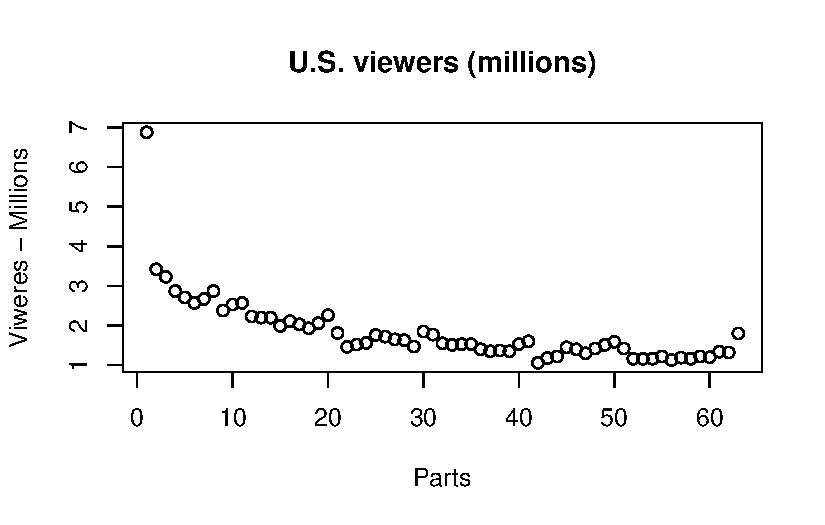
\includegraphics{Le_Nhat_Tung_files/figure-pdf/unnamed-chunk-5-1.pdf}

}

\end{figure}

\hypertarget{u.s.-viewers-millions-over-time-by-season}{%
\subsection{U.S. viewers (millions) over time by
Season}\label{u.s.-viewers-millions-over-time-by-season}}

\begin{Shaded}
\begin{Highlighting}[]
\InformationTok{\textasciigrave{}\textasciigrave{}\textasciigrave{}\{r\}}
\CommentTok{\#| label: fig{-}cars}
\CommentTok{\#| fig{-}cap: "Total Number of Viewers by Season"}
\NormalTok{viewer}\SpecialCharTok{$}\StringTok{\textasciigrave{}}\AttributeTok{U.S. viewers (millions)}\StringTok{\textasciigrave{}} \OtherTok{=} \FunctionTok{as.numeric}\NormalTok{(viewer}\SpecialCharTok{$}\StringTok{\textasciigrave{}}\AttributeTok{U.S. viewers (millions)}\StringTok{\textasciigrave{}}\NormalTok{)}
\FunctionTok{boxplot}\NormalTok{(viewer}\SpecialCharTok{$}\StringTok{\textasciigrave{}}\AttributeTok{U.S. viewers (millions)}\StringTok{\textasciigrave{}} \SpecialCharTok{\textasciitilde{}}\NormalTok{ viewer}\SpecialCharTok{$}\NormalTok{Season, }\AttributeTok{xlab =} \StringTok{"Parts"}\NormalTok{ , }\AttributeTok{ylab =} \StringTok{"Viweres {-} Millions"}\NormalTok{, }\AttributeTok{main =} \StringTok{"U.S. viewers (millions)"}\NormalTok{)}
\InformationTok{\textasciigrave{}\textasciigrave{}\textasciigrave{}}
\end{Highlighting}
\end{Shaded}

\begin{figure}[H]

{\centering 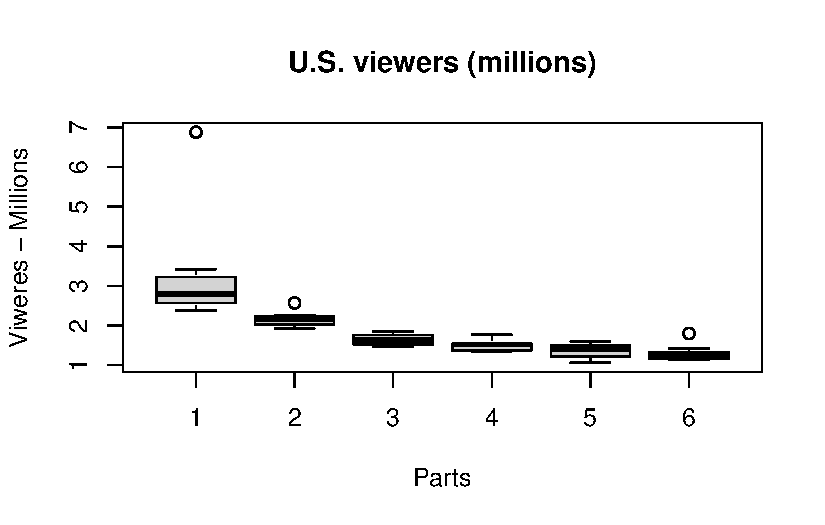
\includegraphics{Le_Nhat_Tung_files/figure-pdf/fig-cars-1.pdf}

}

\caption{\label{fig-cars}Total Number of Viewers by Season}

\end{figure}

Figure~\ref{fig-cars} display total number over viewers by seasons. We
can easly see that the number of viewers dropped dramatically from
season 1 to season 6.



\end{document}
